\chapter{Présentation Générale et Étude de l'Existant}
\label{chap:presentation-etude-existant}

\section*{Introduction}

Ce premier chapitre constitue le socle de notre rapport de projet de fin d'études. Il vise à présenter le cadre général du stage, à savoir l'entreprise d'accueil, les projets sur lesquels nous avons travaillé, ainsi que l'architecture technique existante. Nous procéderons ensuite à une étude critique de l'existant en matière de tests logiciels, ce qui nous permettra de formuler la problématique et de proposer une solution adaptée. Enfin, nous exposerons la méthodologie de travail adoptée tout au long du stage.

%% ====================================================================
%%  1.1 — Présentation de l'entreprise d'accueil
%% ====================================================================
\section{Présentation de l'entreprise d'accueil}
\label{sec:presentation-entreprise}

\subsection{Présentation générale}
\label{subsec:presentation-generale-entreprise}

\textbf{DevWise} est une startup tunisienne basée à Nabeul, spécialisée dans la transformation digitale des entreprises. Fondée avec la conviction que la technologie doit être un levier de croissance accessible à toutes les organisations, DevWise accompagne ses clients dans la conception, le développement et le déploiement de solutions numériques sur mesure.

L'entreprise se distingue par son expertise dans le développement d'applications web et mobiles, en s'appuyant sur des technologies modernes et des méthodologies agiles. DevWise intervient principalement dans les domaines du commerce électronique, de la logistique et de la gestion d'entreprise.

\subsection{Fiche signalétique}
\label{subsec:fiche-signaletique}

Le tableau~\ref{tab:fiche-signaletique} résume les informations clés de l'entreprise d'accueil.

\begin{table}[H]
\centering
\caption{Fiche signalétique de DevWise}
\label{tab:fiche-signaletique}
\begin{tabular}{|l|l|}
\hline
\rowcolor{gray!20}
\textbf{Désignation} & \textbf{Description} \\
\hline
Raison sociale & DevWise \\
\hline
Forme juridique & Startup / SARL \\
\hline
Siège social & Nabeul, Tunisie \\
\hline
Secteur d'activité & Développement logiciel et transformation digitale \\
\hline
Domaines d'expertise & Applications web, applications mobiles, cloud \\
\hline
Technologies principales & Spring Boot, Angular, Flutter, Google Cloud \\
\hline
\end{tabular}
\end{table}

\subsection{Structure organisationnelle}
\label{subsec:structure-organisationnelle}

L'équipe de DevWise est organisée selon une structure horizontale favorisant la collaboration et l'agilité. Elle se compose de~:

\begin{itemize}
    \item \textbf{Direction technique~:} responsable de la vision technologique, de l'architecture logicielle et des choix stratégiques en matière d'outils et de frameworks.
    \item \textbf{Équipe de développement back-end~:} chargée de la conception et de l'implémentation des microservices, des API REST et de la logique métier côté serveur.
    \item \textbf{Équipe de développement front-end~:} responsable du développement des interfaces utilisateur web (Angular) et mobiles (Flutter).
    \item \textbf{Équipe DevOps~:} en charge de l'infrastructure cloud, de l'intégration continue, du déploiement continu et de la supervision des environnements de production.
    \item \textbf{Équipe qualité et tests~:} dédiée à l'assurance qualité, aux tests fonctionnels et à la validation des livrables.
\end{itemize}

\subsection{Valeurs et mission}
\label{subsec:valeurs-mission}

DevWise s'appuie sur un ensemble de valeurs fondamentales qui guident son activité quotidienne~:

\begin{itemize}
    \item \textbf{Innovation~:} adopter les technologies les plus récentes et les meilleures pratiques de l'industrie pour offrir des solutions performantes.
    \item \textbf{Qualité~:} garantir un niveau de qualité élevé à travers des processus rigoureux de développement et de tests.
    \item \textbf{Agilité~:} s'adapter rapidement aux besoins changeants des clients grâce à une méthodologie itérative.
    \item \textbf{Collaboration~:} favoriser le travail d'équipe et la communication transparente entre toutes les parties prenantes.
\end{itemize}

La mission de DevWise est d'accompagner les entreprises tunisiennes et internationales dans leur transformation digitale en leur fournissant des solutions logicielles fiables, évolutives et centrées sur l'utilisateur.

%% ====================================================================
%%  1.2 — Présentation des projets
%% ====================================================================
\section{Présentation des projets}
\label{sec:presentation-projets}

Durant notre stage, nous avons travaillé sur deux projets complémentaires développés par DevWise~: la plateforme \textbf{Speed Line} et l'écosystème \textbf{Delivery App}. Ces deux projets forment ensemble une solution complète de gestion commerciale et de livraison.

\subsection{Speed Line}
\label{subsec:speed-line}

Speed Line est une plateforme de gestion d'entreprise conçue pour centraliser et automatiser les processus métier liés à la gestion commerciale. Elle offre un ensemble complet de fonctionnalités permettant aux entreprises de gérer efficacement leurs opérations quotidiennes.

\subsubsection{Fonctionnalités principales}

Les principales fonctionnalités de Speed Line sont les suivantes~:

\begin{itemize}
    \item \textbf{Gestion des commandes~:} création, suivi et historique des commandes avec gestion des statuts en temps réel.
    \item \textbf{Gestion des clients~:} répertoire complet des clients avec historique d'achats, préférences et informations de contact.
    \item \textbf{Gestion des livreurs~:} affectation des livreurs, suivi de leurs performances et gestion de leur disponibilité.
    \item \textbf{Facturation~:} génération automatique des factures, gestion des paiements et suivi comptable.
    \item \textbf{Tracking en temps réel~:} suivi géolocalisé des livraisons avec notifications en temps réel.
    \item \textbf{Back-office d'administration~:} tableau de bord complet pour la supervision de l'ensemble des opérations.
\end{itemize}

\subsubsection{Stack technique}

Le tableau~\ref{tab:stack-technique-speedline} présente les technologies utilisées dans le développement de Speed Line.

\begin{table}[H]
\centering
\caption{Stack technique de Speed Line}
\label{tab:stack-technique-speedline}
\begin{tabular}{|l|l|l|}
\hline
\rowcolor{gray!20}
\textbf{Couche} & \textbf{Technologie} & \textbf{Version / Détails} \\
\hline
Back-end & Spring Boot (Java) & Java 17, architecture microservices \\
\hline
Front-end (Admin) & Angular & Panel d'administration \\
\hline
Base de données relationnelle & PostgreSQL & Données transactionnelles \\
\hline
Cache & Redis & Sessions, cache applicatif \\
\hline
Infrastructure cloud & Google Cloud & Cloud Run, Pub/Sub \\
\hline
Conteneurisation & Docker & Images de déploiement \\
\hline
CI/CD & GitLab CI & Pipelines automatisés \\
\hline
Gestion de code & Git / GitLab & Versionnement et collaboration \\
\hline
\end{tabular}
\end{table}

\subsection{Delivery App}
\label{subsec:delivery-app}

Delivery App est un écosystème complet de livraison composé de quatre applications distinctes, chacune destinée à un acteur spécifique de la chaîne de livraison. Ensemble, ces applications couvrent l'intégralité du cycle de vie d'une commande, depuis la passation par le client jusqu'à la confirmation de la livraison.

\subsubsection{Application Client (Flutter)}
\label{subsubsec:app-client}

L'application client est développée en \textbf{Flutter} et s'adresse aux utilisateurs finaux. Elle leur permet de~:

\begin{itemize}
    \item Parcourir les catalogues des partenaires et consulter les menus.
    \item Passer des commandes en quelques étapes simples.
    \item Suivre en temps réel l'état de la livraison sur une carte interactive.
    \item Effectuer des paiements en ligne de manière sécurisée.
    \item Consulter l'historique des commandes et laisser des avis.
\end{itemize}

\subsubsection{Application Partenaire (Angular)}
\label{subsubsec:app-partenaire}

L'application partenaire est une application web développée en \textbf{Angular}. Elle est destinée aux restaurants et commerces partenaires et offre les fonctionnalités suivantes~:

\begin{itemize}
    \item Gérer les commandes entrantes (acceptation, préparation, expédition).
    \item Administrer les menus, les produits et les prix.
    \item Suivre les statuts des commandes en temps réel.
    \item Consulter les statistiques de vente et les rapports de performance.
\end{itemize}

\subsubsection{Application Livreur (Flutter)}
\label{subsubsec:app-livreur}

L'application livreur est développée en \textbf{Flutter} et permet aux livreurs de~:

\begin{itemize}
    \item Recevoir les missions de livraison avec les détails de la commande.
    \item Consulter l'itinéraire optimal via une carte intégrée.
    \item Mettre à jour le statut de la livraison en temps réel.
    \item Confirmer la livraison auprès du client.
    \item Consulter l'historique des livraisons effectuées et les gains associés.
\end{itemize}

\subsubsection{Application Admin (Angular)}
\label{subsubsec:app-admin}

L'application d'administration est une application web développée en \textbf{Angular} qui offre une vision globale de l'écosystème. Elle permet de~:

\begin{itemize}
    \item Superviser l'ensemble des commandes, des livraisons et des utilisateurs.
    \item Gérer les comptes des partenaires et des livreurs.
    \item Configurer les paramètres système (zones de livraison, tarification, promotions).
    \item Analyser les performances à travers des tableaux de bord et des rapports détaillés.
    \item Gérer le support client et les réclamations.
\end{itemize}

La figure~\ref{fig:ecosysteme-delivery} illustre les interactions entre les quatre applications de l'écosystème Delivery App.

\begin{figure}[H]
\centering
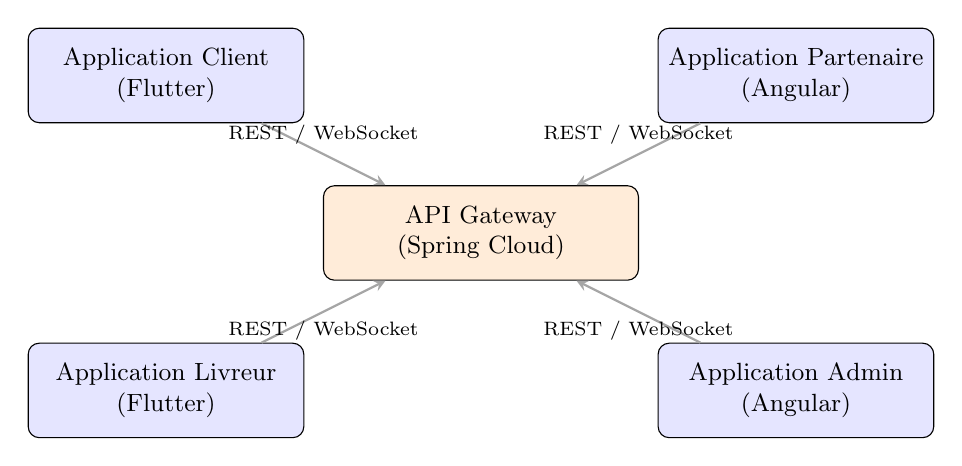
\begin{tikzpicture}[
    app/.style={draw, rounded corners, fill=blue!10, minimum width=3.5cm, minimum height=1.2cm, align=center, font=\small},
    backend/.style={draw, rounded corners, fill=orange!15, minimum width=4cm, minimum height=1.2cm, align=center, font=\small},
    arrow/.style={->, >=stealth, thick, gray!70}
]

% Applications
\node[app] (client) at (-4, 2) {Application Client\\(Flutter)};
\node[app] (partenaire) at (4, 2) {Application Partenaire\\(Angular)};
\node[app] (livreur) at (-4, -2) {Application Livreur\\(Flutter)};
\node[app] (admin) at (4, -2) {Application Admin\\(Angular)};

% Backend
\node[backend] (api) at (0, 0) {API Gateway\\(Spring Cloud)};

% Arrows
\draw[arrow] (client) -- (api);
\draw[arrow] (partenaire) -- (api);
\draw[arrow] (livreur) -- (api);
\draw[arrow] (admin) -- (api);

% Labels on arrows
\node[font=\scriptsize, above, sloped] at (-2, 1) {REST / WebSocket};
\node[font=\scriptsize, above, sloped] at (2, 1) {REST / WebSocket};
\node[font=\scriptsize, below, sloped] at (-2, -1) {REST / WebSocket};
\node[font=\scriptsize, below, sloped] at (2, -1) {REST / WebSocket};

\end{tikzpicture}
\caption{Écosystème Delivery App -- Interactions entre les applications}
\label{fig:ecosysteme-delivery}
\end{figure}

%% ====================================================================
%%  1.3 — Architecture technique existante
%% ====================================================================
\section{Architecture technique existante}
\label{sec:architecture-technique}

L'architecture technique des projets Speed Line et Delivery App repose sur une approche microservices, où chaque service est responsable d'un domaine métier bien défini. Cette section détaille les différents composants de cette architecture.

\subsection{Inventaire des microservices}
\label{subsec:inventaire-microservices}

Le système est composé de douze microservices, chacun encapsulant une responsabilité métier spécifique. Le tableau~\ref{tab:inventaire-services} présente l'inventaire complet de ces services.

\begin{table}[H]
\centering
\caption{Inventaire des microservices}
\label{tab:inventaire-services}
\begin{tabular}{|l|p{8cm}|}
\hline
\rowcolor{gray!20}
\textbf{Microservice} & \textbf{Responsabilité} \\
\hline
\texttt{auth-service} & Authentification, autorisation, gestion des tokens JWT et OAuth2 \\
\hline
\texttt{user-service} & Gestion des profils utilisateurs, préférences et données personnelles \\
\hline
\texttt{partner-service} & Gestion des partenaires (restaurants, commerces), leurs menus et catalogues \\
\hline
\texttt{order-service} & Cycle de vie des commandes, de la création à la clôture \\
\hline
\texttt{delivery-service} & Affectation des livreurs, gestion des tournées et suivi des livraisons \\
\hline
\texttt{payment-service} & Traitement des paiements, facturation et gestion des transactions \\
\hline
\texttt{notification-service} & Envoi de notifications push, SMS et e-mails aux différents acteurs \\
\hline
\texttt{location-service} & Géolocalisation en temps réel, calcul d'itinéraires et zones de couverture \\
\hline
\texttt{analytics-service} & Collecte et analyse des données métier, génération de rapports \\
\hline
\texttt{promotion-service} & Gestion des promotions, codes promo et offres spéciales \\
\hline
\texttt{review-service} & Gestion des avis, notes et retours des utilisateurs \\
\hline
\texttt{support-service} & Support client, gestion des tickets et des réclamations \\
\hline
\end{tabular}
\end{table}

\subsection{Composants d'infrastructure}
\label{subsec:composants-infrastructure}

En plus des microservices métier, l'architecture repose sur plusieurs composants d'infrastructure essentiels~:

\begin{itemize}
    \item \textbf{API Gateway (Spring Cloud Gateway)~:} point d'entrée unique pour toutes les requêtes clients. Il assure le routage, l'équilibrage de charge et la gestion des CORS\footnote{Cross-Origin Resource Sharing.}.
    \item \textbf{Eureka Server (Service Discovery)~:} registre de services permettant la découverte dynamique des microservices et l'équilibrage de charge côté client.
    \item \textbf{Config Server (Spring Cloud Config)~:} serveur de configuration centralisé permettant de gérer les propriétés de tous les services depuis un dépôt Git unique.
\end{itemize}

\subsection{Technologies d'infrastructure}
\label{subsec:technologies-infrastructure}

L'infrastructure de production s'appuie sur les services Google Cloud et plusieurs technologies complémentaires~:

\begin{itemize}
    \item \textbf{Google Cloud Run~:} hébergement des microservices sous forme de conteneurs serverless, offrant une mise à l'échelle automatique.
    \item \textbf{PostgreSQL~:} base de données relationnelle principale pour les données transactionnelles (commandes, utilisateurs, paiements).
    \item \textbf{MongoDB~:} base de données NoSQL utilisée pour les données semi-structurées (logs, historiques de géolocalisation).
    \item \textbf{Redis~:} système de cache en mémoire pour les sessions, les données fréquemment consultées et la gestion des files d'attente.
    \item \textbf{ClickHouse~:} base de données analytique colonnes utilisée par l'\texttt{analytics-service} pour les requêtes agrégées à haute performance.
    \item \textbf{Google Pub/Sub~:} système de messagerie asynchrone pour la communication événementielle entre microservices.
\end{itemize}

\subsection{Pipeline CI/CD}
\label{subsec:pipeline-cicd}

Le déploiement est automatisé grâce à un pipeline CI/CD basé sur \textbf{GitLab CI} et \textbf{Docker}. Le processus suit les étapes suivantes~:

\begin{enumerate}
    \item \textbf{Build~:} compilation du code source et construction de l'image Docker.
    \item \textbf{Tests unitaires~:} exécution des tests existants (avant notre intervention, cette étape était très limitée).
    \item \textbf{Push de l'image~:} publication de l'image Docker sur le registre Google Container Registry.
    \item \textbf{Déploiement~:} déploiement automatique sur Google Cloud Run.
\end{enumerate}

\subsection{Diagramme d'architecture}
\label{subsec:diagramme-architecture}

La figure~\ref{fig:architecture-microservices} présente une vue d'ensemble de l'architecture microservices, illustrant les interactions entre les différents composants du système.

\begin{figure}[H]
\centering
\resizebox{\textwidth}{!}{%
\begin{tikzpicture}[
    service/.style={draw, rounded corners, fill=blue!8, minimum width=2.8cm, minimum height=1cm, align=center, font=\scriptsize\ttfamily},
    infra/.style={draw, rounded corners, fill=green!10, minimum width=2.8cm, minimum height=1cm, align=center, font=\scriptsize\bfseries},
    db/.style={draw, cylinder, shape border rotate=90, aspect=0.25, fill=yellow!15, minimum width=2cm, minimum height=1cm, align=center, font=\scriptsize},
    gateway/.style={draw, rounded corners, fill=red!10, minimum width=3.5cm, minimum height=1cm, align=center, font=\scriptsize\bfseries},
    client/.style={draw, rounded corners, fill=purple!10, minimum width=2.5cm, minimum height=0.9cm, align=center, font=\scriptsize},
    arrow/.style={->, >=stealth, thick, gray!60},
    darrow/.style={<->, >=stealth, thick, gray!60},
    groupbox/.style={draw, dashed, rounded corners, gray!50, inner sep=10pt}
]

% --- Clients (top) ---
\node[client] (c1) at (-5, 8) {App Client\\(Flutter)};
\node[client] (c2) at (-1.5, 8) {App Partenaire\\(Angular)};
\node[client] (c3) at (2, 8) {App Livreur\\(Flutter)};
\node[client] (c4) at (5.5, 8) {App Admin\\(Angular)};

% --- API Gateway ---
\node[gateway] (gw) at (0, 6) {API Gateway};

% --- Infrastructure services ---
\node[infra] (eureka) at (-5.5, 6) {Eureka Server};
\node[infra] (config) at (5.5, 6) {Config Server};

% --- Microservices (two rows) ---
% Row 1
\node[service] (auth) at (-5, 4) {auth-service};
\node[service] (user) at (-2, 4) {user-service};
\node[service] (partner) at (1, 4) {partner-service};
\node[service] (order) at (4, 4) {order-service};

% Row 2
\node[service] (delivery) at (-5, 2.5) {delivery-service};
\node[service] (payment) at (-2, 2.5) {payment-service};
\node[service] (notif) at (1, 2.5) {notification-service};
\node[service] (location) at (4, 2.5) {location-service};

% Row 3
\node[service] (analytics) at (-3.5, 1) {analytics-service};
\node[service] (promo) at (-0.5, 1) {promotion-service};
\node[service] (review) at (2.5, 1) {review-service};
\node[service] (support) at (5.5, 1) {support-service};

% --- Messaging ---
\node[infra] (pubsub) at (0, -0.8) {Google Pub/Sub};

% --- Databases (bottom) ---
\node[db] (pg) at (-4.5, -2.5) {PostgreSQL};
\node[db] (mongo) at (-1.5, -2.5) {MongoDB};
\node[db] (redis) at (1.5, -2.5) {Redis};
\node[db] (click) at (4.5, -2.5) {ClickHouse};

% --- Client to Gateway ---
\foreach \c in {c1, c2, c3, c4}
    \draw[arrow] (\c) -- (gw);

% --- Gateway to services ---
\foreach \s in {auth, user, partner, order}
    \draw[arrow] (gw) -- (\s);

% --- Gateway to second row (indirect via first row, simplified) ---
\draw[arrow, gray!40] (gw.south) -- ++(0,-0.3) -| (delivery.north);
\draw[arrow, gray!40] (gw.south) -- ++(0,-0.3) -| (location.north);

% --- Eureka connections ---
\draw[darrow, dashed, green!50!black] (eureka) -- (gw);
\draw[darrow, dashed, green!50!black] (eureka) -- (auth);

% --- Config connections ---
\draw[darrow, dashed, green!50!black] (config) -- (gw);
\draw[darrow, dashed, green!50!black] (config) -- (order);

% --- Services to Pub/Sub ---
\foreach \s in {order, delivery, payment, notif, location}
    \draw[arrow, blue!40] (\s) -- (pubsub);

% --- Services to Databases ---
\draw[arrow, orange!60] (auth.south) -- ++(0, -0.3) -| (pg);
\draw[arrow, orange!60] (user.south) -- ++(0, -0.3) -| (pg);
\draw[arrow, orange!60] (order.south) -- ++(0, -0.6) -| (pg);
\draw[arrow, orange!60] (location.south) -- ++(0, -0.3) -| (mongo);
\draw[arrow, orange!60] (analytics.south) -- ++(0, -0.3) -| (click);
\draw[arrow, orange!60] (auth.south) -- ++(0, -0.5) -| (redis);

% --- Group boxes ---
\node[groupbox, fit=(auth)(user)(partner)(order)(delivery)(payment)(notif)(location)(analytics)(promo)(review)(support), label={[font=\footnotesize\bfseries, gray]above left:Microservices métier}] {};

\node[groupbox, fit=(pg)(mongo)(redis)(click), label={[font=\footnotesize\bfseries, gray]below:Couche de persistance}] {};

\end{tikzpicture}
}%
\caption{Architecture microservices de Speed Line et Delivery App}
\label{fig:architecture-microservices}
\end{figure}

%% ====================================================================
%%  1.4 — Étude de l'existant -- Tests actuels
%% ====================================================================
\section{Étude de l'existant~: état des tests}
\label{sec:etude-existant-tests}

Avant notre intervention, l'état des tests au sein des projets Speed Line et Delivery App présentait des lacunes importantes. Cette section dresse un bilan complet de la couverture de tests existante et identifie les problèmes qui en découlent.

\subsection{Couverture de tests avant le stage}
\label{subsec:couverture-tests-avant}

Le tableau~\ref{tab:couverture-tests-avant} présente l'état de la couverture de tests pour chaque microservice avant le début du stage. On constate une disparité significative entre les services, avec une majorité de services ne disposant que d'un nombre minimal, voire nul, de fichiers de tests.

\begin{table}[H]
\centering
\caption{Couverture de tests par microservice avant le stage}
\label{tab:couverture-tests-avant}
\begin{tabular}{|l|c|c|l|}
\hline
\rowcolor{gray!20}
\textbf{Microservice} & \textbf{Fichiers de tests} & \textbf{Couverture estimée} & \textbf{Observation} \\
\hline
\texttt{auth-service} & 2 & $< 5\%$ & Tests basiques uniquement \\
\hline
\texttt{user-service} & 1 & $< 3\%$ & Quasi inexistant \\
\hline
\texttt{partner-service} & 1 & $< 3\%$ & Quasi inexistant \\
\hline
\texttt{order-service} & 2 & $< 5\%$ & Tests minimaux \\
\hline
\texttt{delivery-service} & \textbf{41} & $\sim 35\%$ & Le plus couvert \\
\hline
\texttt{payment-service} & 0 & $0\%$ & Aucun test \\
\hline
\texttt{notification-service} & 0 & $0\%$ & Aucun test \\
\hline
\texttt{location-service} & 1 & $< 3\%$ & Quasi inexistant \\
\hline
\texttt{analytics-service} & 0 & $0\%$ & Aucun test \\
\hline
\texttt{promotion-service} & \textbf{20} & $\sim 20\%$ & Partiellement couvert \\
\hline
\texttt{review-service} & 0 & $0\%$ & Aucun test \\
\hline
\texttt{support-service} & 0 & $0\%$ & Aucun test \\
\hline
\rowcolor{blue!5}
\textbf{Total} & \textbf{68} & $\sim 5\%$ (moyenne) & \textbf{Très insuffisant} \\
\hline
\end{tabular}
\end{table}

\subsection{Types de tests absents}
\label{subsec:types-tests-absents}

Au-delà du faible nombre de tests unitaires, plusieurs catégories de tests étaient totalement absentes~:

\begin{itemize}
    \item \textbf{Tests de bout en bout (E2E)~:} aucun scénario de test simulant le parcours complet d'un utilisateur n'était en place.
    \item \textbf{Tests d'API~:} aucune suite de tests automatisés ne validait le comportement des endpoints REST des microservices.
    \item \textbf{Tests de performance~:} aucun test de charge ou de stress n'avait été réalisé pour évaluer la tenue en charge du système.
    \item \textbf{Tests mobiles~:} les applications Flutter (client et livreur) ne disposaient d'aucun test automatisé, ni unitaire ni d'intégration.
    \item \textbf{Tests d'intégration~:} les interactions entre microservices n'étaient pas testées de manière automatisée.
\end{itemize}

\subsection{Conséquences observées}
\label{subsec:consequences-observees}

L'absence quasi totale de tests automatisés engendrait plusieurs problèmes opérationnels majeurs~:

\begin{enumerate}
    \item \textbf{Bugs en production~:} des anomalies étaient régulièrement détectées par les utilisateurs finaux en environnement de production, ce qui nuisait à l'expérience utilisateur et à la crédibilité du produit.
    \item \textbf{Tests manuels chronophages~:} chaque nouvelle fonctionnalité ou correction de bug nécessitait une phase de test manuelle longue et fastidieuse, ralentissant considérablement le cycle de livraison.
    \item \textbf{Absence de détection de régressions~:} sans tests automatisés, il était impossible de détecter automatiquement les régressions introduites par de nouvelles modifications du code.
    \item \textbf{Confiance réduite dans les déploiements~:} l'équipe de développement manquait de confiance lors des mises en production, ce qui entraînait soit des retards, soit des déploiements risqués.
    \item \textbf{Dette technique croissante~:} l'accumulation de code non testé rendait la maintenance et l'évolution du système de plus en plus difficiles.
\end{enumerate}

%% ====================================================================
%%  1.5 — Problématique
%% ====================================================================
\section{Problématique}
\label{sec:problematique}

À la lumière de l'étude de l'existant, nous pouvons formuler la problématique suivante~:

\begin{quote}
\textit{Comment assurer la qualité logicielle et la fiabilité d'un écosystème distribué composé de douze microservices et de quatre applications front-end, dans un contexte de développement rapide et de déploiements fréquents, tout en réduisant les risques de régression et en accélérant le cycle de livraison~?}
\end{quote}

Cette problématique se décline en plusieurs défis concrets~:

\begin{itemize}
    \item \textbf{Complexité architecturale~:} le système repose sur douze microservices interconnectés, chacun avec sa propre base de données et sa propre logique métier. La surface de test est donc considérable.
    \item \textbf{Diversité technologique~:} l'écosystème comprend deux applications Angular et deux applications Flutter, nécessitant des outils et des approches de test différents.
    \item \textbf{Tests manuels inadaptés~:} avec la croissance du code source et la fréquence des déploiements, les tests manuels deviennent trop lents et sujets aux erreurs humaines.
    \item \textbf{Absence d'intégration CI/CD~:} les tests existants ne sont pas intégrés dans le pipeline de déploiement, ce qui signifie que du code non testé peut être déployé en production.
    \item \textbf{Risque de régression~:} chaque modification du code dans un service peut avoir des répercussions sur d'autres services, et sans tests automatisés, ces régressions passent inaperçues.
\end{itemize}

%% ====================================================================
%%  1.6 — Solution proposée
%% ====================================================================
\section{Solution proposée}
\label{sec:solution-proposee}

Pour répondre à la problématique identifiée, nous proposons la mise en place d'un \textbf{robot de tests automatisés} couvrant l'ensemble de la pyramide de tests. Cette solution s'articule autour de quatre axes principaux correspondant aux quatre niveaux de la pyramide de tests logiciels.

\subsection{Pyramide de tests}
\label{subsec:pyramide-tests}

Notre solution couvre les quatre couches de la pyramide de tests, comme illustré dans la figure~\ref{fig:pyramide-tests}~:

\begin{figure}[H]
\centering
\begin{tikzpicture}[
    layer/.style={trapezium, trapezium angle=75, draw, minimum height=1cm, align=center, font=\small},
]

% Pyramid layers (bottom to top)
\node[layer, fill=green!20, minimum width=10cm] (unit) at (0, 0) {\textbf{Tests unitaires} -- JUnit 5, Mockito, Flutter test};
\node[layer, fill=blue!15, minimum width=7.5cm] (integration) at (0, 1.5) {\textbf{Tests d'intégration} -- Spring Boot Test, Testcontainers};
\node[layer, fill=orange!15, minimum width=5cm] (api) at (0, 3) {\textbf{Tests API} -- Playwright API Testing};
\node[layer, fill=red!15, minimum width=3cm] (e2e) at (0, 4.5) {\textbf{Tests E2E} -- Playwright, Patrol};

% Annotations
\node[right, font=\scriptsize, gray] at (5.5, 0) {Rapides, nombreux, isolés};
\node[right, font=\scriptsize, gray] at (4.2, 1.5) {Interactions entre composants};
\node[right, font=\scriptsize, gray] at (3, 3) {Validation des endpoints};
\node[right, font=\scriptsize, gray] at (2, 4.5) {Scénarios utilisateur};

% Side label
\draw[<->, thick, gray] (-6, -0.5) -- (-6, 5) node[midway, left, font=\footnotesize, align=center, rotate=90] {Coût et temps d'exécution};

\end{tikzpicture}
\caption{Pyramide de tests -- Solution proposée}
\label{fig:pyramide-tests}
\end{figure}

\subsection{Axes de la solution}
\label{subsec:axes-solution}

\begin{enumerate}
    \item \textbf{Tests unitaires (couche de base)~:} écriture de tests unitaires pour chaque microservice à l'aide de JUnit~5 et Mockito. Ces tests valident le comportement isolé de chaque composant (services, contrôleurs, utilitaires). Pour les applications Flutter, nous utiliserons le framework de test natif.

    \item \textbf{Tests d'intégration~:} mise en place de tests d'intégration avec Spring Boot Test et Testcontainers pour valider les interactions entre les composants au sein d'un même service (base de données, cache, messaging).

    \item \textbf{Tests API~:} développement d'une suite complète de tests API avec Playwright pour valider le comportement des endpoints REST de chaque microservice.

    \item \textbf{Tests de bout en bout (E2E)~:} automatisation des scénarios utilisateur complets avec Playwright pour les applications web (Angular) et Patrol pour les applications mobiles (Flutter).
\end{enumerate}

\subsection{Tests de performance}
\label{subsec:tests-performance}

En complément de la pyramide de tests, nous intégrerons des \textbf{tests de performance} à l'aide de l'outil \textbf{k6}. Ces tests permettront de~:

\begin{itemize}
    \item Mesurer les temps de réponse des API sous charge.
    \item Identifier les goulots d'étranglement.
    \item Valider la capacité du système à supporter un volume d'utilisateurs simultanés conforme aux exigences.
\end{itemize}

\subsection{Intégration CI/CD}
\label{subsec:integration-cicd-solution}

L'ensemble des tests sera intégré dans le pipeline CI/CD de GitLab CI. Chaque commit et chaque merge request déclenchera automatiquement l'exécution des tests pertinents, empêchant le déploiement de code non conforme.

\subsection{Rapports visuels}
\label{subsec:rapports-visuels}

Nous mettrons en place des rapports de tests visuels à l'aide d'\textbf{Allure Report}, offrant~:

\begin{itemize}
    \item Un tableau de bord interactif avec le taux de réussite global.
    \item Le détail de chaque test (durée, résultat, captures d'écran en cas d'échec).
    \item L'historique des exécutions pour suivre l'évolution de la couverture.
    \item Des graphiques de tendance pour identifier les tests instables.
\end{itemize}

%% ====================================================================
%%  1.7 — Méthodologie de travail
%% ====================================================================
\section{Méthodologie de travail}
\label{sec:methodologie-travail}

\subsection{Approche Agile / Scrum}
\label{subsec:approche-agile}

Pour mener à bien ce projet, nous avons adopté la méthodologie \textbf{Agile Scrum}, une approche itérative et incrémentale particulièrement adaptée aux projets de développement logiciel. Cette méthodologie nous permet de~:

\begin{itemize}
    \item Livrer des incréments fonctionnels à intervalles réguliers.
    \item S'adapter aux changements de priorités et aux retours des parties prenantes.
    \item Maintenir une communication constante avec l'équipe de développement.
    \item Mesurer la progression du projet de manière continue.
\end{itemize}

Les cérémonies Scrum suivantes ont été mises en place~:

\begin{itemize}
    \item \textbf{Sprint Planning~:} planification des tâches au début de chaque sprint (durée de 2 semaines).
    \item \textbf{Daily Standup~:} réunion quotidienne de synchronisation avec l'équipe.
    \item \textbf{Sprint Review~:} démonstration des résultats à la fin de chaque sprint.
    \item \textbf{Sprint Retrospective~:} analyse de ce qui a bien fonctionné et identification des axes d'amélioration.
\end{itemize}

\subsection{Planning prévisionnel}
\label{subsec:planning-previsionnel}

Le stage s'étend sur une durée de quatre mois, organisés en huit sprints de deux semaines chacun. Le tableau~\ref{tab:planning-sprints} présente le planning prévisionnel.

\begin{table}[H]
\centering
\caption{Planning prévisionnel des sprints}
\label{tab:planning-sprints}
\begin{tabular}{|c|l|p{7cm}|}
\hline
\rowcolor{gray!20}
\textbf{Sprint} & \textbf{Période} & \textbf{Objectifs} \\
\hline
1 & Semaines 1--2 & Prise en main du projet, étude de l'existant, mise en place de l'environnement de tests \\
\hline
2 & Semaines 3--4 & Tests unitaires -- \texttt{auth-service}, \texttt{user-service}, \texttt{partner-service} \\
\hline
3 & Semaines 5--6 & Tests unitaires -- \texttt{order-service}, \texttt{delivery-service}, \texttt{payment-service} \\
\hline
4 & Semaines 7--8 & Tests unitaires -- services restants + tests d'intégration \\
\hline
5 & Semaines 9--10 & Tests API avec Playwright pour les services critiques \\
\hline
6 & Semaines 11--12 & Tests E2E -- applications Angular (Admin, Partenaire) \\
\hline
7 & Semaines 13--14 & Tests E2E -- applications Flutter (Client, Livreur) + tests de performance (k6) \\
\hline
8 & Semaines 15--16 & Intégration CI/CD, rapports Allure, documentation et finalisation \\
\hline
\end{tabular}
\end{table}

\subsection{Outils de travail}
\label{subsec:outils-travail}

Le tableau~\ref{tab:outils-travail} récapitule les principaux outils utilisés au cours du stage.

\begin{table}[H]
\centering
\caption{Outils de travail}
\label{tab:outils-travail}
\begin{tabular}{|l|l|p{6cm}|}
\hline
\rowcolor{gray!20}
\textbf{Catégorie} & \textbf{Outil} & \textbf{Utilisation} \\
\hline
Gestion de code & Git / GitLab & Versionnement, branches, merge requests \\
\hline
Tests unitaires (Java) & JUnit 5, Mockito & Tests des microservices Spring Boot \\
\hline
Tests unitaires (Flutter) & Flutter Test, Patrol & Tests des applications mobiles \\
\hline
Tests d'intégration & Spring Boot Test & Tests avec contexte applicatif \\
\hline
Tests d'intégration & Testcontainers & Bases de données conteneurisées pour les tests \\
\hline
Tests API & Playwright & Validation automatisée des endpoints REST \\
\hline
Tests E2E (Web) & Playwright & Automatisation des navigateurs web \\
\hline
Tests E2E (Mobile) & Patrol & Automatisation des applications Flutter \\
\hline
Tests de performance & k6 & Tests de charge et de stress \\
\hline
Rapports & Allure Report & Génération de rapports visuels interactifs \\
\hline
CI/CD & GitLab CI & Automatisation du pipeline de tests \\
\hline
Conteneurisation & Docker & Environnements de tests isolés \\
\hline
\end{tabular}
\end{table}

%% ====================================================================
%%  Conclusion du chapitre
%% ====================================================================
\section*{Conclusion}

Dans ce premier chapitre, nous avons présenté l'entreprise d'accueil DevWise ainsi que les deux projets sur lesquels porte notre stage~: Speed Line et Delivery App. L'étude de l'architecture technique existante a révélé un écosystème riche composé de douze microservices et de quatre applications front-end. L'analyse de l'état des tests a mis en lumière des lacunes importantes, avec une couverture globale estimée à seulement 5\%, l'absence totale de tests E2E, de tests API et de tests de performance, et aucune intégration des tests dans le pipeline CI/CD.

Face à cette problématique, nous avons proposé une solution basée sur la pyramide de tests, couvrant les tests unitaires, les tests d'intégration, les tests API et les tests E2E, le tout intégré dans le pipeline CI/CD avec des rapports visuels Allure. La méthodologie Agile Scrum adoptée nous permettra de mener à bien ce projet de manière itérative sur une durée de quatre mois.

Le chapitre suivant sera consacré à l'état de l'art, où nous étudierons les concepts fondamentaux des tests logiciels et les outils que nous utiliserons.
